\chapter{자외선 발산과 초대칭에 의한 해결}

\lectureoverview{초대칭의 형식적 수학을 소개하기 전에, 초대칭이 해결하려는 문제가 무엇인지 정확히 짚어 둘 필요가 있다. 위치 공간과 운동량 공간에서 자외선 발산을 설명하고, 차원 분석으로 스칼라와 페르미온 전파자의 단거리 거동을 유도한 뒤, 스칼라 질량에 대한 주요 루프 보정을 추정하겠다. 스칼라 루프와 페르미온 루프는 차단 운동량에 대해 같은 이차 의존성을 가지지만 부호는 반대다. 두 기여의 결합 상수, 다중도, 질량이 우연한 상쇄가 아니라 구조적인 상쇄가 일어날 만큼 서로 잘 맞도록 하는 원리가 무엇인지 물으면 초대칭의 필요성이 분명해진다.}

\section{발산을 왜 다시 살펴보는가?}

원래는 초대칭의 수학적 기법을 곧바로 시작하려 했다. 하지만 한 강의 동안 추상적인 논의를 미루고 동기를 다시 살펴보는 편이 낫다. 앞서 발산과 질량 재규격화에 관한 설명은 빠르게 지나갔다. 무엇을 바로잡아야 하는지 정확히 살펴보지 않으면 초대칭은 자의적인 수학적 발명처럼 보일 것이다.

파인만 도표는 서로 밀접한 두 방식으로 입자물리학에 쓰인다. 가장 익숙한 용도는 산란 진폭을 체계적으로 정리하는 것이다. 입사 입자와 출사 입자를 지정한 다음, 필요한 차수의 모든 도표가 나타내는 진폭을 합한다. 파인만 도표는 \emph{유효 라그랑지언}을 구성할 때도 쓰인다. 여기서 ``유효''라는 말은 특별히 성공적이라는 칭찬이 아니다. 기술이 근사적이라는 뜻이다. 접근할 수 없는 단거리 세부 사항은 제거하거나 적분해 없애고, 그 영향은 남은 매개변수와 상호작용에 담는다.

모든 기술에는 유효 범위가 있다. 이 범위는 여기서 \(\delta\)로 나타내는, 신뢰할 수 있는 최단 거리로 지정할 수도 있고, 신뢰할 수 있는 최대 운동량으로 지정할 수도 있다.
\begin{equation}
\Lambda\sim \delta^{-1}.
\end{equation}
두 차단 척도는 별개의 가정이 아니다. 같은 자외선 극한을 푸리에 변환으로 표현한 두 가지 방식이다.

\section{전파자 하나, 두 가지 기술}

전파자는 한 시공간 점에서 입자를 만들거나 삽입하고 다른 점에서 제거하거나 검출하는 진폭이다. 두 점을 \(x^\mu\)와 \(y^\mu\)라 하고, 두 점 사이의 차이를 다음과 같이 쓰자.
\begin{equation}
\Delta^\mu=y^\mu-x^\mu.
\end{equation}
분리 거리와 조절 변수가 혼동되지 않도록 차단 척도에는 소문자 기호 \(\delta\)를 사용한다.

병진 대칭성에 따르면 자유 전파자는 \(x\)와 \(y\)에 각각 의존하지 않고, 오직 \(\Delta\)를 통해서만 의존한다. 같은 대상을 푸리에 변환할 수도 있다.
\begin{equation}
G(\Delta)
=\int\frac{d^4k}{(2\pi)^4}\,e^{-ik\cdot\Delta}\,\widetilde G(k).
\end{equation}

``위치의 푸리에 켤레 변수는 무엇인가?''라고 강의실에 물으면 답은 운동량이다. 따라서 루프를 출발점으로 되돌아오는 전파자로 기술하는 위치 공간의 설명은, 루프를 따라 흐를 수 있는 모든 운동량에 대해 적분하는 운동량 공간의 설명과 동등하다. 운동량 공간의 규칙에서는 각 꼭짓점에서 운동량 보존을 적용해야 한다. 위치 공간에서는 지금 다루는 거듭제곱 계수 계산을 더 분명하게 볼 수 있다.

이 등가성 덕분에 계산을 시작하기도 전에 자외선 문제가 무엇인지 알 수 있다. 위치 공간에서 루프는 두 점이 일치하는 극한 \(\Delta\to0\)을 살핀다. 운동량 공간에서는 \(|k|\to\infty\)의 극한을 살핀다. 큰 운동량은 짧은 파장을 뜻하므로, 단거리 특이점과 고운동량 발산은 서로 다른 좌표로 표현한 같은 현상이다.

이 강의에서는 가장 단순한 스핀 계, 즉 스칼라장과 페르미온장을 다루고, 게이지장은 배경으로 언급한다. 스칼라의 스핀은 0이며 한 성분으로 된 장 \(\phi(x)\)으로 나타낸다. 강의가 녹화된 2010 당시에는 힉스가 아직 발견되지 않았고, 입자물리학에서 예상되는 주요 스칼라 입자로 설명되었다. 그런 시대적 배경 때문에 ``힉글리위글리''라는 장난스러운 표현이 등장한다. 이 장은 물리적으로 중요한 관심사였지만 실험으로는 아직 확인되지 않았다.

실수 스칼라장의 전파자는 개략적으로 다음과 같이 쓸 수 있다.
\begin{equation}
G_\phi(x,y)=\expect{0|T\!\left\{\phi(x)\phi(y)\right\}|0}
=G_\phi(\Delta).
\end{equation}
시간 순서화 규약과 정규화는 거듭제곱 계수 계산에 영향을 주지 않는다. 중요한 점은 두 장 삽입이 한 점에서의 생성과 다른 점에서의 소멸을 나타낸다는 것이다.

\begin{classroomqa}
\audiencequestion{\(x\)와 \(y\)는 공간상의 위치인가, 시공간상의 위치인가? \lecturetimestamp{00:09:31}}
\lecturerresponse{시공간상의 점이다. 각각은 사차원 벡터다. 따라서 전파자는 두 점 사이의 사차원 분리에 의존하며, 로런츠 불변 진공에서는 그에 대응하는 불변 간격에 의존한다.}
\end{classroomqa}

스핀 1/2 입자는 디랙 장 \(\psi_i(x)\)으로 기술된다. 지수 \(i\)는 스피너 지수이지 공간 성분이 아니므로, 전파자는 행렬이다:
\begin{equation}
S_{ij}(x,y)=\expect{0|T\!\left\{\psi_i(x)\bar\psi_j(y)\right\}|0}
=S_{ij}(\Delta).
\end{equation}

강의실에 던진 질문을 통해 성분 수를 확인한다. 사차원 디랙장에는 복소 성분이 네 개 있다. 질량이 없는 바일장은 복소 성분 두 개로 기술할 수 있으므로, 왼손잡이장과 오른손잡이장을 따로 다룰 수 있다. 지금의 차원 논증에서는 스피너 행렬 구조가 존재한다는 점만 중요하다.

\(S_{ij}\)는 \(4\times4\) 행렬이므로 디랙 행렬의 기저로 전개할 수 있다. 우선 그 첨자들은 생략하고, 필요해지면 다시 표시하겠다. 행렬 구조가 없다고 주장하는 것이 아니다. 자외선에서의 거듭제곱 법칙을 세우는 동안 의도적으로 단순화하는 것이다.

\begin{classroomqa}
\audiencequestion{전파자에서 켤레장 또는 에르미트 수반장이 필요한 경우는 언제인가? \lecturetimestamp{00:14:06}}
\lecturerresponse{이 개략적인 논의에서 실수 중성 스칼라는 같은 장에 생성 연산자와 소멸 연산자가 들어 있으므로, 별도의 에르미트 수반장이 필요하지 않다. 하전장의 경우에는 입자와 반입자 연산자를 구별해야 한다. 따라서 전자에서는 \(\psi\), \(\psi^\dagger\), 그리고 공변적으로 정의한 \(\bar\psi=\psi^\dagger\gamma^0\)가 서로 다른 역할을 한다.}
\end{classroomqa}

물리적인 힉스 입자는 중성이지만, 그 바탕이 되는 표준 모형의 힉스장은 전약 이중항이다. 이 강의에서는 실수 중성 스칼라를 국소적인 모형으로 사용하며, 자외선 거동을 추정하기에는 이 단순화로 충분하다.\editorialnote{이 구분을 통해 개략적인 실수 스칼라의 예를 전약 힉스 다중항에 관한 완전한 설명으로 오해하지 않도록 한다.}

\section{자연 단위계와 스칼라장의 차원}

\(\hbar=c=1\)로 둔다. 그러면 길이와 시간은 같은 단위를 가지며, 에너지와 질량, 운동량의 단위는 길이의 역수다.
\begin{equation}
[m]=[E]=[p]=L^{-1}.
\end{equation}
작용은 위상 \(e^{iS}\)에 들어가므로 무차원이다. 시공간이 사차원일 때 스칼라장의 대표적인 작용은 다음과 같다.
\begin{equation}
S_\phi=\int d^4x\left[
\frac12\partial_\mu\phi\,\partial^\mu\phi
-\frac12m^2\phi^2
-\frac{\lambda}{4!}\phi^4
+\cdots\right].
\end{equation}
관례적으로 들어가는 \(1/2\)와 \(1/4!\)는 차원 분석에 영향을 주지 않는다.

운동항부터 살펴보자. \([d^4x]=L^4\)이고 \([\partial_\mu]=L^{-1}\)이므로, 작용이 무차원이라는 조건에서 다음을 얻는다.
\begin{align}
1
&=L^4\left(L^{-1}[\phi]\right)^2,\\
[\phi]&=L^{-1}.
\end{align}
질량항으로 확인할 수도 있다.
\begin{equation}
L^4[m^2][\phi^2]
=L^4L^{-2}L^{-2}=1.
\end{equation}

다음으로 강의실에 물은 것은 사차 상호작용 결합 상수의 차원이다. 시공간이 사차원일 때 이 결합 상수는 무차원이다.
\begin{equation}
L^4[\lambda][\phi]^4=L^4[\lambda]L^{-4}=1
\quad\Longrightarrow\quad [\lambda]=L^0.
\end{equation}
따라서 사차원에서는 \(\phi^4\) 상호작용이 특별하다. \(\phi^6\) 및 그보다 높은 차수의 상호작용 차원도 같은 규칙으로 구할 수 있지만, 그 결합 상수에는 질량의 음의 거듭제곱이 들어가므로 유효 이론에서의 적용 범위가 더 제한적임을 알 수 있다.

이처럼 장의 차원만으로도 어떤 상호작용이 무차원 계수를 가질 수 있는지 알 수 있다. 같은 방법으로 자세한 파인만 적분을 계산하지 않고도 전파자와 유카와 결합의 차원을 구할 수 있다.

\section{단거리에서의 스칼라 전파자}

먼저 질량이 없는 스칼라를 생각하자. 고유한 길이 척도가 없으므로 사용할 수 있는 유일한 척도는 분리 거리 \(\Delta\)다. 병진 대칭성 때문에 의존성은 \(\Delta\)에만 남고, 로런츠 대칭성은 이를 불변 크기에 대한 의존성으로 줄인다. 스칼라장 두 개의 곱은 \(L^{-2}\)의 차원을 가지므로, 수치 상수를 제외하면
\begin{equation}
G_0(\Delta)\sim\frac{1}{\Delta^2}.
\end{equation}
\(4\pi^2\) 같은 인자는 차원 논증만으로는 정할 수 없다.

질량은 콤프턴 길이 \(m^{-1}\)를 도입한다. 그 효과는 분산 관계를 보면 가장 쉽게 이해할 수 있다.
\begin{equation}
E=\sqrt{\bm p^{,2}+m^2},
\qquad
E=|\bm p|\quad(m=0).
\end{equation}
\(|\bm p|\gg m\)일 때 질량은 무시할 수 있다. 고운동량은 단거리를 살피므로, 질량이 있는 전파자는 \(\Delta\to0\)일 때 질량 없는 경우의 \(1/\Delta^2\) 거동에 가까워져야 한다. \(m^{-1}\)보다 훨씬 먼 거리에서는 전파가 억제된다. 강의에서는 이를 개략적으로 다음과 같이 나타낸다.
\begin{equation}
G_m(\Delta)\sim \frac{e^{-m|\Delta|}}{\Delta^2}.
\end{equation}
이 식은 의도적으로 정확한 식이 아닌 개략적인 표현이다. 사차원 유클리드 공간에서 정확한 자유 전파자는 \(mK_1(mr)/r\)에 비례하고, 여기서 \(r=|\Delta|\)이다. 이 전파자도 같은 \(1/r^2\) 자외선 특이점을 가지며, 큰 거리에서는 거듭제곱 전인자가 곱해진 지수적 감소를 보인다.\editorialnote{베셀 함수 형태는 강의에서 개략적으로 나타낸 지수 함수를 표준적인 정확한 식으로 완성한다. 다만 거듭제곱 계수 세기(power counting) 논증에는 이 식이 필요하지 않다.}

핵심은 간단하다. 질량은 장거리 전파를 약화하지만, 두 점이 일치할 때의 특이점은 없애지 못한다. 한 점에 충분히 가까우면 유한한 질량은 모두 무시할 수 있다.

\section{스칼라 타드폴과 미세 조정}

사차 상호작용 \(\lambda\phi^4\)은 선 네 개가 만나는 꼭짓점을 만든다. 그중 두 선을 서로 연결하고, 나머지 두 선은 외부 스칼라 다리로 둔다. 이렇게 얻는 타드폴 도표는 \(\phi^2\)의 계수를 보정하므로 스칼라 질량 제곱에 영향을 준다.

보존된 강의 프레임에는 차원 분석에서 이 루프 보정으로 넘어가는 순간이 정확히 담겨 있다. 왼쪽에는 분산 관계가 남아 있고 오른쪽에는 스칼라 작용과 장의 차원이 일부 보이며, 가운데에는 작은 타드폴 도표가 막 나타났다.

\begin{figure}[H]
\centering
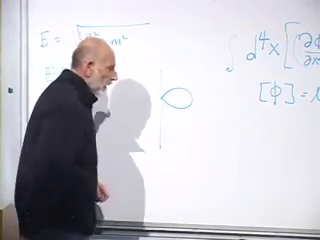
\includegraphics[width=0.72\textwidth]{lecture_03_figure_02.png}
\lectureframe{00:28:30.560}

\medskip
\begin{tikzpicture}[line width=0.8pt,scale=1.0]
  \draw[dashed] (-2.6,0) -- (0,0) -- (2.6,0);
  \fill (0,0) circle (0.055);
  \draw (0,0) .. controls (-0.85,0.7) and (-0.85,1.6) .. (0,1.6)
                .. controls (0.85,1.6) and (0.85,0.7) .. (0,0);
\end{tikzpicture}
\caption{스칼라 자기 에너지 논의로 넘어가는 순간의 칠판 모습과, 타드폴 도표의 위상만 보수적으로 다시 그린 그림이다. 스크린샷에서는 루프와 상대론적·질량 없는 에너지 식, 그리고 작용의 일부를 확실히 확인할 수 있다. 가려진 계수와 표기는 보인다고 주장하지 않는다.}
\end{figure}

꼭짓점에서 스칼라가 흡수되었다가 다시 방출되는 동안 다른 두 다리는 그 점에서 출발해 다시 그 점으로 전파될 수 있다. 수치 인자와 조합론적 인자를 제외하면 보정은 다음과 같다.
\begin{equation}
\delta m_\phi^2\sim \lambda G_\phi(0).
\end{equation}
연속체 근사에서 두 점이 일치하는 전파자는 발산한다. 유효 이론은 임의로 짧은 거리까지 유효하다고 주장하지 않으므로, \(|\Delta|\geq\delta\)을 부과하자. 그러면
\begin{equation}
G_\phi(0)\longrightarrow G_\phi(\delta)sim\frac{1}{\delta^2},
\qquad
\delta m_\phi^2\sim\frac{\lambda}{\delta^2}sim\lambda\Lambda^2.
\end{equation}
운동량 차단 척도의 제곱이 들어가므로 이 발산을 이차 발산이라 한다. 운동량 공간에서 적분해도 같은 결론을 얻는다. 지나치게 큰 기여는 한없이 큰 루프 운동량에서 나온다. 최단 거리 척도가 결국 대통일, 양자중력 또는 아직 상상하지 못한 무엇에 의해 정해지는지는 유효 이론의 진단을 바꾸지 않는다.

이는 미세 조정 문제다. \(\delta\)가 극도로 작고 \(\lambda\)가 특별히 미소한 값이 아니라면, 복사 보정은 저에너지에서 관측되는 스칼라 질량 제곱보다 훨씬 크다. 그러면 맨계수와 루프 보정이 믿기 어려울 정도로 많은 자릿수에서 상쇄되어야 한다.
\begin{equation}
m_{\mathrm{physical}}^2
=m_{\mathrm{bare}}^2+\delta m_\phi^2.
\end{equation}
질량이 있는 전파자라고 해서 문제가 해결되지는 않는다. 발산을 일으키는 거리에서는 \(e^{-m|\Delta|}\simeq1\)이다. 자외선 루프는 차단 척도에 도달하기 훨씬 전에 이미 질량을 무시한다.

\section{페르미온의 차원과 전파자}

이제 디랙 페르미온에 대해서도 같은 차원 분석을 해 보자. 자유 작용은 다음과 같다.
\begin{equation}
S_\psi=\int d^4x\,
\bar\psi\left(i\gamma^\mu\partial_\mu-m\right)\psi.
\end{equation}
감마 행렬은 수치로 이루어져 있으며 무차원이다. 운동항에는 미분이 하나만 포함되므로
\begin{align}
1
&=L^4[\bar\psi]L^{-1}[\psi],\\
[\psi]=[\bar\psi]&=L^{-3/2}.
\end{align}
반정수 거듭제곱을 보고 놀랄 필요는 없다. 페르미온 때문에 여러 곳에서 반정수가 나타난다.

\begin{classroomqa}
\audiencequestion{질량항으로 \([\psi]\)를 구하는 편이 더 쉽지 않은가? \lecturetimestamp{00:36:02}}
\lecturerresponse{그렇다. 질량항에서는 \(L^4L^{-1}[\bar\psi\psi]=1\)를 얻으므로, \([\bar\psi\psi]=L^{-3}\)이고 \([\psi]=L^{-3/2}\)이다. 질량이 없는 이론에서도 쓸 수 있고 페르미온 질량이 \(m\)로 나타나는 이유를 보여 주므로, 먼저 운동항을 이용해 유도했다. 페르미온 질량은 \(m^2\)로 나타나지 않는다.}
\end{classroomqa}

페르미온장 두 개의 차원은 \(L^{-3}\)이므로, 질량 없는 전파자에 대한 강의의 간결한 차원 표기는 다음과 같다.
\begin{equation}
S(\Delta)\sim\frac{1}{|\Delta|^3}.
\end{equation}
행렬 구조를 복원하면 로런츠 공변성에 필요한 더 정확한 분자가 나온다.
\begin{equation}
S_{ij}(\Delta)
\propto
\frac{\left(\gamma_\mu\Delta^\mu\right)_{ij}}
{\left(\Delta^2\right)^2}.
\end{equation}
분자에는 길이의 1승이 더해지므로 분모에는 간격의 4승이 들어간다. 전체 차원은 여전히 \(L^{-3}\)이다. 스칼라와 마찬가지로 페르미온 질량은 큰 분리 거리에서 전파자를 억제하지만, 단거리 스케일링은 바꾸지 않는다.

\section{닫힌 페르미온 루프의 부호가 음수인 이유}

이제 페르미온 도표가 문제가 되는 보손 자기 에너지를 상쇄할 수 있는지 물을 수 있다. 스칼라 타드폴의 부호는 \(\pi\)의 거듭제곱이나 조합론적 계수 같은 양의 수치 인자를 제외하면 양수다. 닫힌 페르미온 루프는 반대 부호를 갖는다.

\begin{classroomqa}
\audiencequestion{페르미온 루프의 음의 부호는 앞서 논의한 한 바퀴 회전과 관련이 있는가? \lecturetimestamp{00:40:21}}
\lecturerresponse{같은 페르미온 부호 구조와 관련은 있지만, 여기서는 루프의 기하학적 방향보다 입자 교환 반대칭성을 이용해 증명하는 편이 유용하다. 두 루프를 각각 자르고 동일한 입자들을 서로 교환한 다음 다시 연결하자. 두 루프가 하나로 합쳐지며, 그 교환은 페르미온에서만 음의 부호를 준다.}
\end{classroomqa}

전체 논증을 자세히 제시할 가치가 있다. 한 루프 도표의 부호가 \(\sigma\)이라고 하자. 부호는 양수일 수도 음수일 수도 있다. 서로 연결되지 않은 동일한 두 루프의 부호는 다음과 같다.
\begin{equation}
\sigma^2=+1.
\end{equation}
두 루프를 동시에 절단하자. 그러면 절단면 사이에서 동일한 두 입자가 전파된다. 통상적인 두 입자 파동함수는 보손의 경우 대칭이고 페르미온의 경우 반대칭이다:
\begin{align}
\Psi_B(x_1,x_2)&=+\Psi_B(x_2,x_1),\\
\Psi_F(x_1,x_2)&=-\Psi_F(x_2,x_1).
\end{align}
이 반대칭성은 파울리 원리도 설명한다. 두 페르미온을 같은 상태에 놓으면 서로 교환해도 물리적으로는 변함이 없지만, 파동함수의 부호는 반대가 되어야 하므로 파동함수는 사라진다.

두 입자를 교환한 뒤 절단된 선을 다시 연결하자. 위상적으로 두 루프는 하나가 된다. 교환하지 않은 두 루프 진폭은 양수였다. 교환해도 보손에서는 양의 부호가 유지되지만, 페르미온에서는 부호가 뒤집힌다. 따라서
\begin{equation}
\begin{aligned}
\operatorname{sign}(\text{closed boson loop})&=+1,\\
\operatorname{sign}(\text{closed fermion loop})&=-1.
\end{aligned}
\end{equation}
이는 일반적인 결론이다. 서로 독립적인 닫힌 페르미온 루프마다 \(-1\) 인자가 하나씩 붙는다.

\section{유카와 루프}

스칼라 질량으로 돌아가자. 페르미온 수 패리티가 달라지므로 보손 하나가 페르미온 하나로 바뀔 수는 없다. 가장 단순한 페르미온 보정에서는 스칼라가 페르미온과 반페르미온 쌍으로 갈라지고, 이 쌍이 루프를 따라 전파된 뒤 다시 결합한다. 이 상호작용은 유카와 결합으로 주어진다.
\begin{equation}
\mathcal L_Y=-g\phi\bar\psi\psi.
\end{equation}
힉스의 경우 페르미온은 쿼크나 렙톤일 수 있다. 상호작용점이 두 개이므로 \(g\) 인자도 두 개가 들어간다.

스칼라 타드폴에는 상호작용점이 하나 있었다. 병진 대칭성 때문에 시공간 부피만 곱해지므로 그 점의 전체 위치는 고정할 수 있었다. 유카와 루프에는 점이 두 개 있다. 한 점을 고정하거나, 같은 뜻으로 두 점의 평균 위치를 고정할 수는 있지만, 상대적 분리 \(\Delta\)에 대해서는 적분해야 한다. 각 페르미온 전파자가 단거리 인자 \(1/|\Delta|^3\)를 주므로,
\begin{equation}
\delta m_{\phi,F}^2
\sim
-g^2\int_{|\Delta|\geq\delta}d^4\Delta\,
\frac{1}{|\Delta|^6}.
\end{equation}

두 전파자와 분리 거리 적분, 두 결합을 적은 다음 마지막 인자를 강의실에 물었다. 답은 음의 부호다. 두 전파자가 닫힌 페르미온 루프를 이루므로, 나머지는 모두 양수인 단거리 적분 전체에 \(-1\)가 곱해진다.

발산은 차원 분석만으로 이미 결정된다. \(d^4\Delta\)에서 길이의 4승이 나오고 분모에는 6승이 들어가며, 남는 길이 척도는 차단 척도뿐이다.
\begin{equation}
\int_{|\Delta|\geq\delta}
\frac{d^4\Delta}{|\Delta|^6}
\sim\frac{1}{\delta^2}.
\end{equation}
사차원 유클리드 방사 좌표에서는 이를 명시적으로 나타낼 수 있다.
\begin{equation}
\int_{\delta}^{R}d^4\Delta\,\frac{1}{|\Delta|^6}
=2\pi^2\int_{\delta}^{R}dr\,\frac{r^3}{r^6}
=\pi^2\left(\frac{1}{\delta^2}-\frac{1}{R^2}\right).
\end{equation}
스피너의 대각합과 전파자 정규화는 계수를 바꾸지만 차단 척도에 대한 이차 거듭제곱은 바꾸지 않는다.\editorialnote{방사 적분은 강의에서 제시한 차원 추정을 명시적으로 나타낸 표준적인 예다. 양의 적분 측도와 자외선 거듭제곱 계수를 분명히 볼 수 있도록 유클리드 거리로 썼다.}

\begin{classroomqa}
\audiencequestion{적분 순서를 뒤집거나 적분 구간을 택하는 방식이 부호를 바꿀 수 있는가? \lecturetimestamp{00:51:06}}
\lecturerresponse{아니다. 물리적인 부호가 적분 한계에서 나오는, 방향을 가진 일차원 적분이 아니다. 네 성분에 대한 적분이며, 양의 방사 측도로 쓰면 더 분명하다. 자외선 기여의 크기는 양수다. 음의 기여는 닫힌 페르미온 루프에서만 나온다.}
\end{classroomqa}

\begin{classroomqa}
\audiencequestion{유카와 결합 \(g\)의 차원은 얼마인가? \lecturetimestamp{00:51:51}}
\lecturerresponse{사차원에서 무차원이다. \([\phi]=L^{-1}\)이고 \([\bar\psi\psi]=L^{-3}\)이므로, 곱 \(\phi\bar\psi\psi\)의 차원은 \(L^{-4}\)이다. 이 차원은 \(d^4x\)가 상쇄한다.}
\end{classroomqa}

따라서 페르미온의 주요 보정은 다음과 같다.
\begin{equation}
\delta m_{\phi,F}^2
\sim -C_F\frac{g^2}{\delta^2}
=-C_Fg^2\Lambda^2,
\end{equation}
여기서 \(C_F>0\)에는 수치 인자와 스핀, 다중도 인자가 들어간다. 스칼라 루프의 대응하는 식은 다음과 같다.
\begin{equation}
\delta m_{\phi,B}^2
\sim+C_B\frac{\lambda}{\delta^2}
=+C_B\lambda\Lambda^2.
\end{equation}
아직 미세 조정 문제를 해결하지는 못했지만, 반드시 필요한 사실 하나를 찾았다. 같은 자외선 차수를 가지면서 부호가 반대인 기여가 있다는 것이다.

\section{상쇄에 필요한 조건}

서로 무관한 결합 상수들이 큰 에너지 척도 계층에 필요한 정밀도만큼 정확히 다음 관계를 우연히 만족하는 것은 놀라운 우연일 것이다.
\begin{equation}
C_B\lambda=C_Fg^2
\end{equation}
강의에서는 관례에 따라 달라지는 인자와 다중도 인자를 생략하고 이를 \(g^2=\lambda\)로 줄여 쓴다. 진정한 해결책이라면 단지 그 관계를 허용하는 데 그치지 않고, 수학적 구조로 그 관계가 성립하도록 강제해야 한다.

이것이 초대칭의 동기다. 초대칭은 보손과 페르미온을 서로 연결하고, 위험한 발산 항 다수가 상쇄되도록 결합 상수의 조합을 제한한다. 이 상쇄는 매 루프마다 매개변수를 따로 조정해서 얻는 것이 아니라 대칭성에서 비롯되므로 여러 도표에서 반복된다.

질량의 일치도 중요하다. 보손과 페르미온의 질량이 같으면 전체 전파자를 가장 밀접하게 짝지을 수 있다. 질량이 조금 다르면 콤프턴 파장과 비슷한 거리에서 전파자가 서로 달라지므로 완전한 유한 기여는 정확히 상쇄되지 않는다. 그래도 두 전파자의 공통 단거리 점근 형태는 발산 부분을 상쇄할 수 있다.
\begin{equation}
\mathcal I_B(\Delta)-\mathcal I_F(\Delta)
\quad\hbox{may be finite as}\quad \Delta\to0,
\end{equation}
여기서 \(\mathcal I_B\)와 \(\mathcal I_F\)은 꼭짓점, 분자, 다중도를 포함한 보손 및 페르미온 루프 적분함수 전체를 뜻한다. 차원이 서로 다른 전파자 자체를 직접 빼는 것은 아니다. 자외선 항이 상쇄되어도 유한한 잔여항은 남을 수 있다. 이것이 근사 초대칭 또는 깨진 초대칭으로 이어지는 출발점이다. 정확한 질량 일치는 가장 깔끔한 상쇄를 준다. 충분히 제어된 대칭성 깨짐도 관측 가능한 질량 차이를 남기면서 자외선 재앙을 없앨 수 있다.

이제 초대칭의 대수 구조를 쓰기 전부터 초대칭에 이르렀다. 논리는 다음과 같이 완결된다.
\begin{equation}
\begin{gathered}
G_\phi(\Delta)\sim \Delta^{-2},
\qquad
\delta m_{\phi,B}^2\sim+C_B\lambda\Lambda^2,\\[0.4em]
S_\psi(\Delta)\sim \Delta^{-3},
\qquad
\delta m_{\phi,F}^2\sim-C_Fg^2\Lambda^2,\\[0.4em]
\text{symmetry-enforced matching}\\
\Longrightarrow\quad
\text{quadratic divergences cancel}.
\end{gathered}
\end{equation}
다음으로는 이러한 관계를 강제하는 추상적인 대칭성 원리를 이해하고, 그것이 어떻게 작용하는지 구체적인 예를 살펴보겠다.
